\ifx\allfiles\undefined
\documentclass{XDBAthesis}
\def\pictures{}
\begin{document}
\else
\fi
\chapter{基于OpenCV实现Android系统对摄像头的调用及操作}

\section{OpenCV环境搭建}

在搭建好Android开发坏境的前提下,下载Cygwin,配置NDK。配置好后,下载OpenCV for Android编译,进入Cygwin shell执行(注意路径中的空格):svn checkout http://android-opencv.googlecode.com/svn/trunk/  android-opencv-read-only

    之后进入OpenCV目录执行sh build.sh编译,编译完成后即可以使用Eclipse+ADT的方式完成OpenCV程序的开发。

\section{架构设计}

    在已经搭建好了编译环境后,接下来主要进行两部分的开发:首先主要是涉及 UI 界面和程序的逻辑流程在基于Android应用程序框架下进行Java端的开发;其次是JNI接口的开发,通过OpenCV与JNI接口编写本地的 C/C++ 代码,并利用 Android NDK 对其进行编译,然后运用编译后生成的 Java 代码可调用动态链接库so文件,最后通过 Eclipse 编译打包并生成应用程序,整体框架图如图\ref{fg:whole}所示。
\begin{figure}[htb]
    \centering
    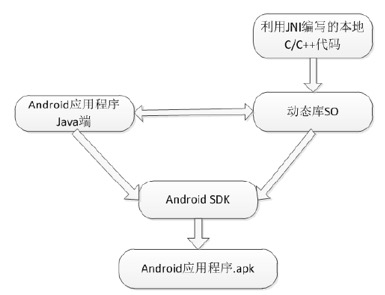
\includegraphics[width=0.8\textwidth]{figure/opencv}
    \caption{整体框架图}
    \label{fg:whole}
\end{figure}


\section{highGUI库函数进行对摄像头的调用及操作}

先建立一个窗口,用来显示图像。通过cvCreateCameraCapture来读取摄像头。该函数的输入参数是一个ID号,只有存在多个摄像头时才起作用。对摄像头成功调用后,可以采取对图像的目标算法来实现对摄像头采集到图像的相应操作。函数cvGrabFrame从摄像头或者文件中抓取帧。被抓取的帧在内部被存储。这个函数的目的是快速的抓取帧,这一点对同时从几个摄像头读取数据的同步是很重要的。

\section{照相机和Opencv同时对摄像头占用的处理方案}

    传统的处理方法是将图像一帧帧传入数据层,数据层调用图像处理函数完成对图像的处理后,再将图像传入表现层,使前端可以显示出当前图像。但是由于CPU有限,处理时间较长,会造成很明显的延时导致用户使用效果不理想。因此针对延时问题,采用多线程处理方案,当摄像头捕捉到图像后,对传入图像进行分频处理,即一帧传入数据层,一帧传入表现层。由于图像捕捉每一帧时间极短,因此在表现层也不会出现断帧的现象。分频处理不单单使画面更加流畅,还使软件在实时性的效果更好,图片处理更加快速。



\ifx\allfiles\undefined
%\bibliographystyle{unsrt}
\bibliography{main}
\end{document}
\fi